\documentclass[11pt,a4paper]{report}
\usepackage[textwidth=37em,vmargin=30mm]{geometry}
\usepackage{calc,xunicode,amsmath,amssymb,paralist,enumitem,tabu,booktabs,datetime2,xeCJK,xeCJKfntef,listings}
\usepackage{tocloft,fancyhdr,tcolorbox,xcolor,graphicx,eso-pic,xltxtra,xelatexemoji}

\newcommand{\envyear}[0]{2025}
\newcommand{\envdatestr}[0]{2025-02-08}
\newcommand{\envfinaldir}[0]{webdb/2025/20250208/final}

\usepackage[hidelinks]{hyperref}
\hypersetup{
    colorlinks=false,
    pdfpagemode=FullScreen,
    pdftitle={Web Digest - \envdatestr}
}

\setlength{\cftbeforechapskip}{10pt}
\renewcommand{\cftchapfont}{\rmfamily\bfseries\large\raggedright}
\setlength{\cftbeforesecskip}{2pt}
\renewcommand{\cftsecfont}{\sffamily\small\raggedright}

\setdefaultleftmargin{2em}{2em}{1em}{1em}{1em}{1em}

\usepackage{xeCJK,xeCJKfntef}
\xeCJKsetup{PunctStyle=plain,RubberPunctSkip=false,CJKglue=\strut\hskip 0pt plus 0.1em minus 0.05em,CJKecglue=\strut\hskip 0.22em plus 0.2em}
\XeTeXlinebreaklocale "zh"
\XeTeXlinebreakskip = 0pt


\setmainfont{Brygada 1918}
\setromanfont{Brygada 1918}
\setsansfont{IBM Plex Sans}
\setmonofont{JetBrains Mono NL}
\setCJKmainfont{Noto Serif CJK SC}
\setCJKromanfont{Noto Serif CJK SC}
\setCJKsansfont{Noto Sans CJK SC}
\setCJKmonofont{Noto Sans CJK SC}

\setlength{\parindent}{0pt}
\setlength{\parskip}{8pt}
\linespread{1.15}

\lstset{
	basicstyle=\ttfamily\footnotesize,
	numbersep=5pt,
	backgroundcolor=\color{black!5},
	showspaces=false,
	showstringspaces=false,
	showtabs=false,
	tabsize=2,
	captionpos=b,
	breaklines=true,
	breakatwhitespace=true,
	breakautoindent=true,
	linewidth=\textwidth
}






\newcommand{\coverpic}[2]{
    % argv: itemurl, authorname
    Cover photo by #2~~(\href{#1}{#1})
}
\newcommand{\makeheader}[0]{
    \begin{titlepage}
        % \newgeometry{hmargin=15mm,tmargin=21mm,bmargin=12mm}
        \begin{center}
            
            \rmfamily\scshape
            \fontspec{BaskervilleF}
            \fontspec{Old Standard}
            \fontsize{59pt}{70pt}\selectfont
            WEB\hfill DIGEST
            
            \vfill
            % \vskip 30pt
            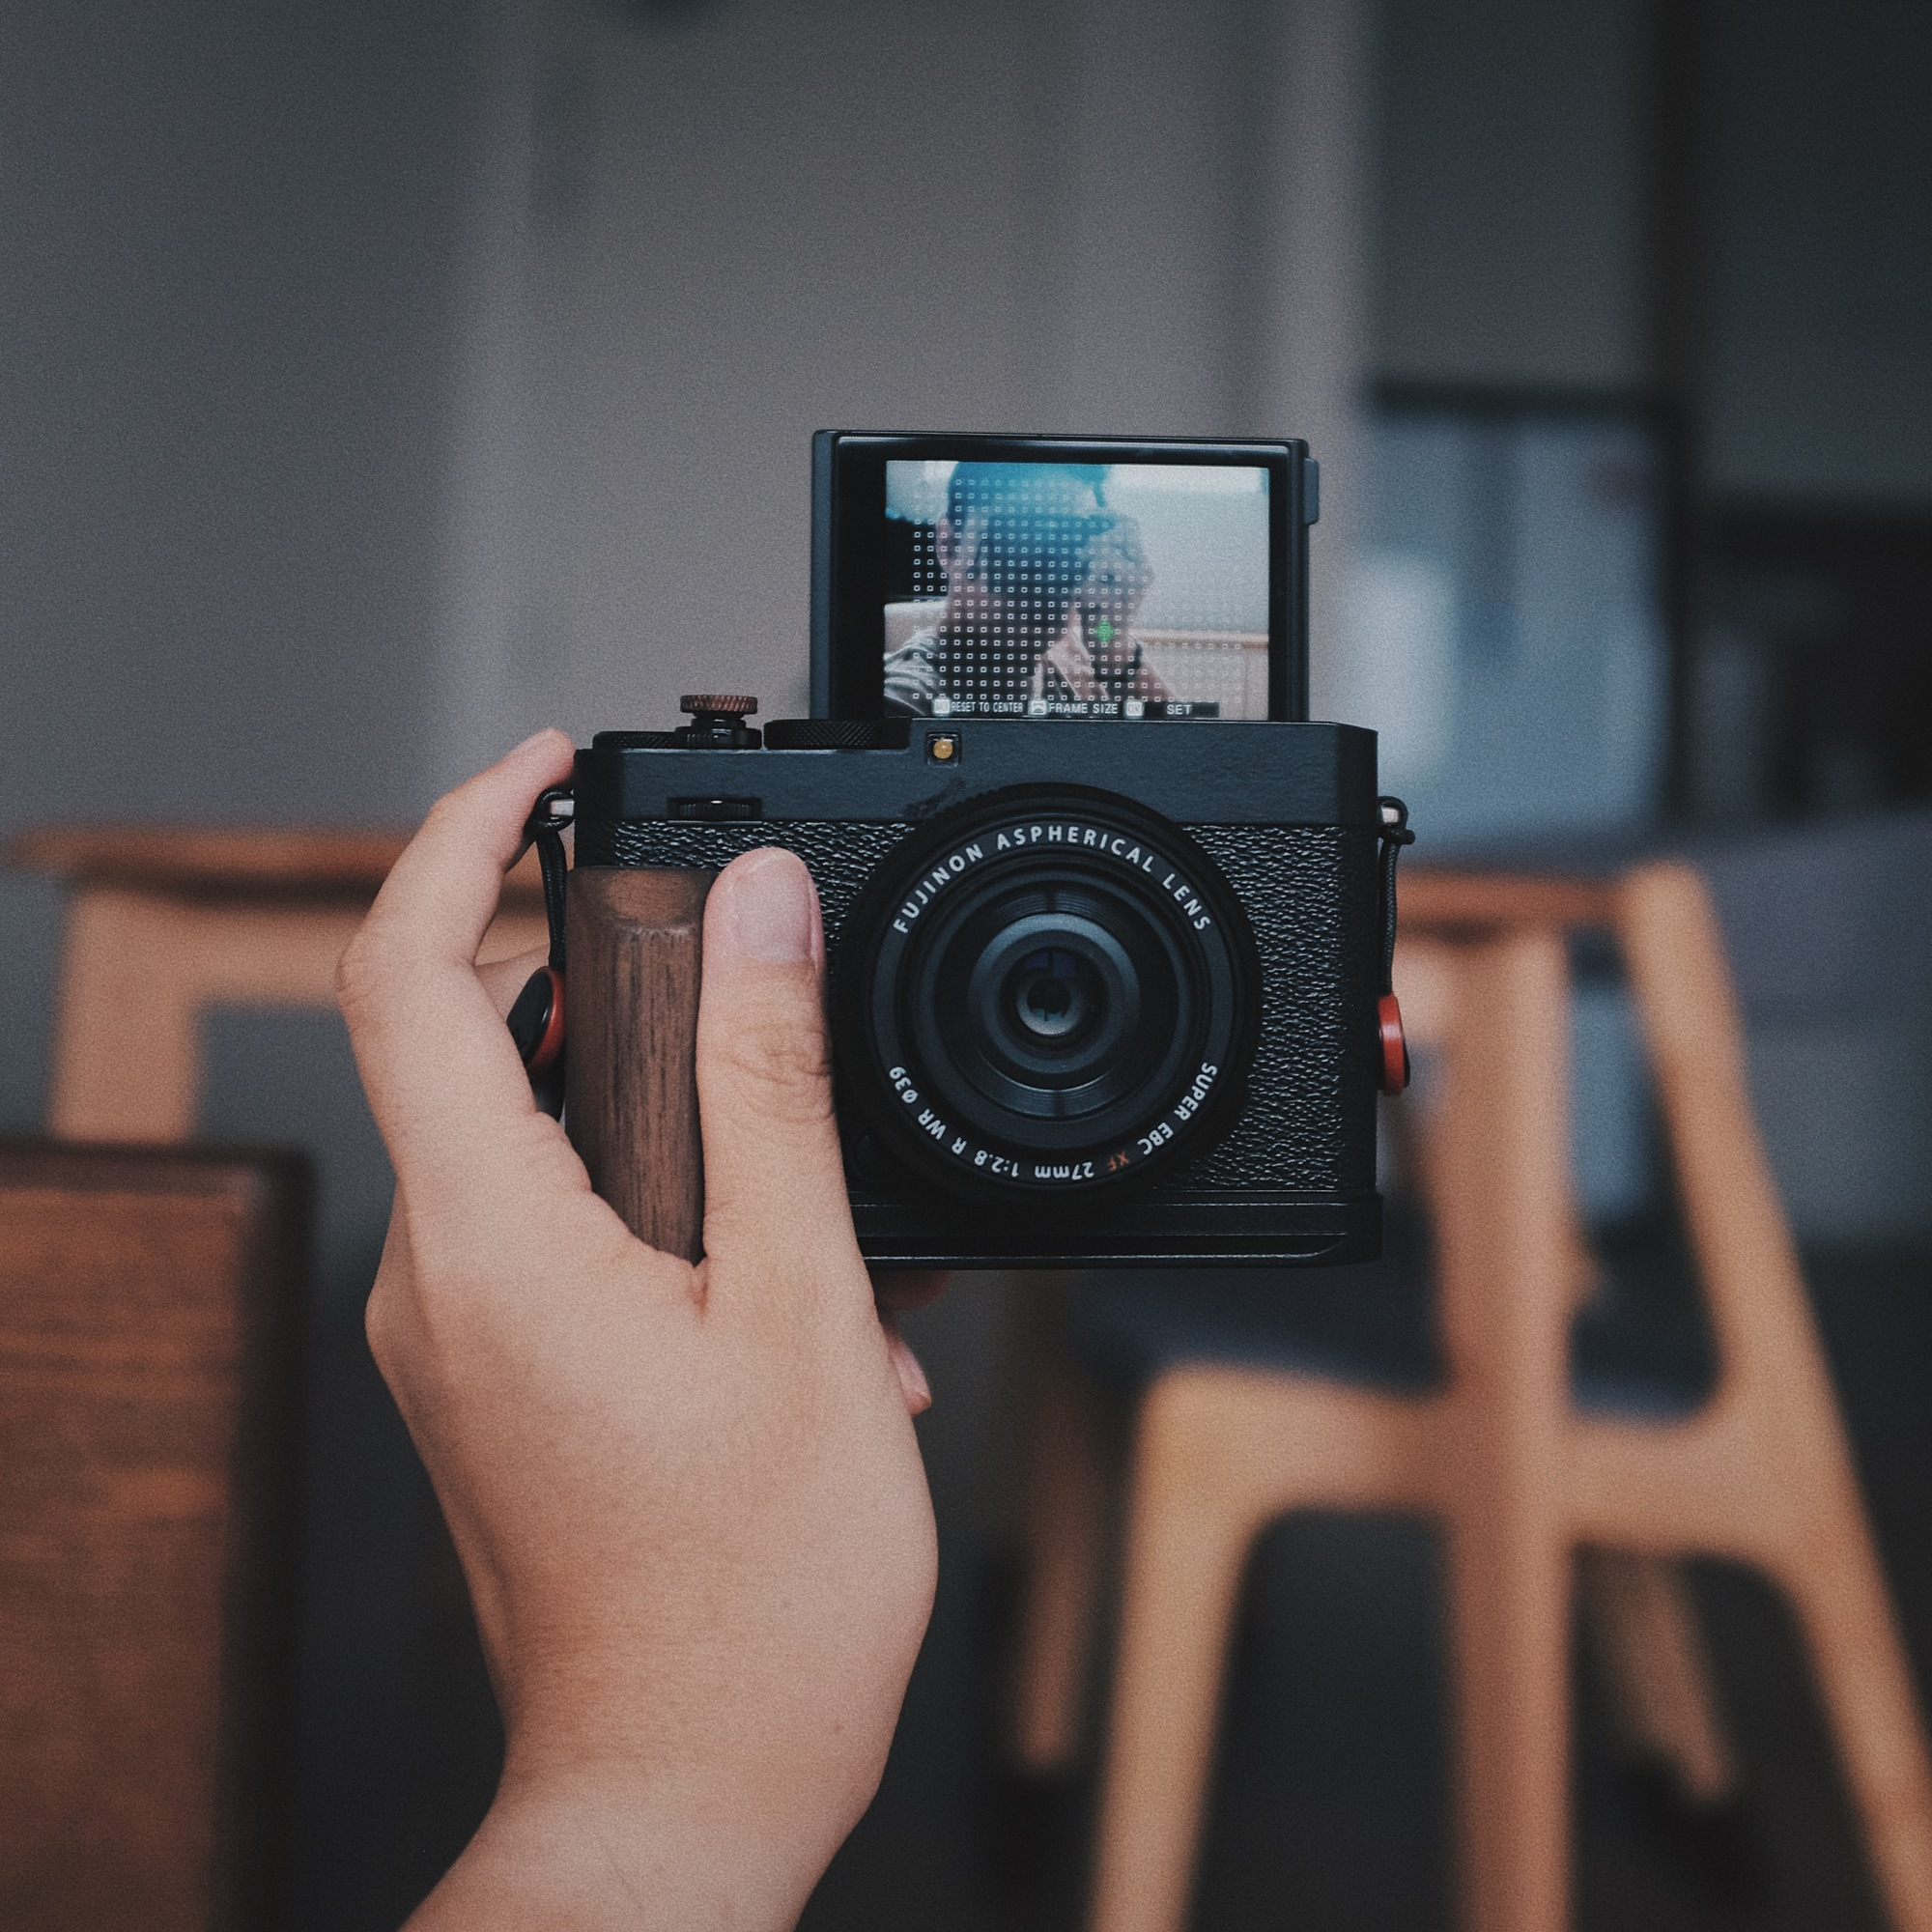
\includegraphics[width=\linewidth]{\envfinaldir/coverpic-prod.jpg}\par
            % \vskip 30pt
            \vfill

            \normalsize\rmfamily\scshape
            \copyright{} The Web Digest Project \hfill\large \envdatestr
        \end{center}
    \end{titlepage}
    % \restoregeometry
}
\newcommand{\simplehref}[1]{%
    \textcolor{blue!80!green}{\href{#1}{#1}}%
}
\renewcommand{\contentsname}{\center\Huge\sffamily\bfseries Contents\par\vskip 20pt}
\newcounter{ipartcounter}
\setcounter{ipartcounter}{0}
\newcommand{\ipart}[1]{
    % \vskip 20pt
    \clearpage
    \stepcounter{ipartcounter}
    \phantomsection
    \addcontentsline{toc}{chapter}{#1}
    % \begin{center}
    %     \Huge
    %     \sffamily\bfseries
    %     #1
    % \end{center}
    % \vskip 20pt plus 7pt
}
\newcounter{ichaptercounter}
\setcounter{ichaptercounter}{0}
\newcommand{\ichapter}[1]{
    % \vskip 20pt
    \clearpage
    \stepcounter{ichaptercounter}
    \phantomsection
    \addcontentsline{toc}{section}{\numberline{\arabic{ichaptercounter}}#1}
    \begin{center}
        \Huge
        \sffamily\bfseries
        #1
    \end{center}
    \vskip 20pt plus 7pt
}
\newcommand{\entrytitlefont}[1]{\subsection*{\raggedright\Large\sffamily\bfseries#1}}
\newcommand{\entryitemGeneric}[2]{
    % argv: title, url
    \parbox{\linewidth}{
        \entrytitlefont{#1}\par\vskip 5pt
        \footnotesize\ttfamily\mdseries
        \simplehref{#2}
    }\vskip 11pt plus 11pt minus 1pt
}
\newcommand{\entryitemGithub}[3]{
    % argv: title, url, desc
    \parbox{\linewidth}{
        \entrytitlefont{#1}\par\vskip 5pt
        \footnotesize\ttfamily\mdseries
        \simplehref{#2}\par\vskip 5pt
        \small\rmfamily\mdseries#3
    }\vskip 11pt plus 11pt minus 1pt
}
\newcommand{\entryitemAp}[3]{
    % argv: title, url, desc
    \parbox{\linewidth}{
        \entrytitlefont{#1}\par\vskip 5pt
        \footnotesize\ttfamily\mdseries
        \simplehref{#2}\par\vskip 5pt
        \small\rmfamily\mdseries#3
    }\vskip 11pt plus 11pt minus 1pt
}
\newcommand{\entryitemHackernews}[3]{
    % argv: title, hnurl, rawurl
    % \parbox{\linewidth}{
    %     \entrytitlefont{#1}\par\vskip 5pt
    %     \footnotesize\ttfamily\mdseries
    %     \simplehref{#3}\par
    %     \textcolor{black!50}{\href{#2}{#2}}
    % }\vskip 11pt plus 11pt minus 1pt
    \begin{minipage}{\linewidth}
            \entrytitlefont{#1}\par\vskip 5pt
            \footnotesize\ttfamily\mdseries
            \simplehref{#3}\par
            \textcolor{black!50}{\href{#2}{#2}}
    \end{minipage}\par\vskip 11pt plus 11pt minus 1pt
}







\begin{document}

\makeheader

\tableofcontents\clearpage




\ipart{Developers}
\ichapter{Hacker News}
\entryitemTwoLinks{Show HN: A website that heatmaps your city based on your housing preferences}{https://news.ycombinator.com/item?id=42975803}{https://theretowhere.com/}

\entryitemTwoLinks{A brief history of code signing at Mozilla}{https://news.ycombinator.com/item?id=42975436}{https://hearsum.ca/posts/history-of-code-signing-at-mozilla/}

\entryitemTwoLinks{A German court rules: X must provide researchers access to data}{https://news.ycombinator.com/item?id=42975170}{https://www.reuters.com/world/europe/german-civil-activists-claim-victory-case-against-musks-x-2025-02-07/}

\entryitemTwoLinks{The origins of 60-Hz as a power frequency}{https://news.ycombinator.com/item?id=42974809}{https://ieeexplore.ieee.org/document/628099}

\entryitemTwoLinks{Stop using zip codes for geospatial analysis (2019)}{https://news.ycombinator.com/item?id=42974728}{https://carto.com/blog/zip-codes-spatial-analysis}

\entryitemTwoLinks{A 16TB Mirror of Data.gov on Source.Coop}{https://news.ycombinator.com/item?id=42974533}{https://source.coop/repositories/harvard-lil/gov-data/description}

\entryitemTwoLinks{Three-nanite: Unreal Nanite in Three.js}{https://news.ycombinator.com/item?id=42974461}{https://github.com/AIFanatic/three-nanite}

\entryitemTwoLinks{Show HN: Transductive regular expressions for text editing}{https://news.ycombinator.com/item?id=42974378}{https://github.com/c0stya/trre}

\entryitemTwoLinks{Kokoro WebGPU: Real-time text-to-speech 100\% locally in the browser}{https://news.ycombinator.com/item?id=42973769}{https://huggingface.co/spaces/webml-community/kokoro-webgpu}

\entryitemTwoLinks{Baltic countries disconnect from the Russian power grid}{https://news.ycombinator.com/item?id=42973131}{https://baltic-grid.sympower.net/}

\entryitemTwoLinks{Asahi Linux lead developer Hector Martin resigns from Linux kernel}{https://news.ycombinator.com/item?id=42972062}{https://lkml.org/lkml/2025/2/7/9}

\entryitemTwoLinks{Whalesong patterns follow a universal law of human language, new research finds}{https://news.ycombinator.com/item?id=42971847}{https://theconversation.com/whalesong-patterns-follow-a-universal-law-of-human-language-new-research-finds-249271}

\entryitemTwoLinks{Apple Ordered by UK to Create Global iCloud Encryption Backdoor}{https://news.ycombinator.com/item?id=42971761}{https://www.macrumors.com/2025/02/07/uk-government-orders-access-icloud/}

\entryitemTwoLinks{Meta torrented \& seeded 81.7 TB dataset containing copyrighted data}{https://news.ycombinator.com/item?id=42971446}{https://arstechnica.com/tech-policy/2025/02/meta-torrented-over-81-7tb-of-pirated-books-to-train-ai-authors-say/}

\entryitemTwoLinks{Copilot stops working on code that contains hardcoded banned words from GitHub (2023)}{https://news.ycombinator.com/item?id=42971279}{https://github.com/orgs/community/discussions/72603}

\entryitemTwoLinks{Shwe Kokko is accused of being a city built on scams}{https://news.ycombinator.com/item?id=42971059}{https://www.bbc.co.uk/news/articles/c04nx1vnw17o}

\entryitemTwoLinks{U.K. orders Apple to let it spy on users' encrypted accounts}{https://news.ycombinator.com/item?id=42970412}{https://www.washingtonpost.com/technology/2025/02/07/apple-encryption-backdoor-uk/}

\entryitemTwoLinks{Donald Knuth's 2024 Christmas Lecture: Strong and Weak Components [video]}{https://news.ycombinator.com/item?id=42970240}{https://www.youtube.com/watch?v=Hi8r\_63LGyg}

\entryitemTwoLinks{Announcing the data.gov archive}{https://news.ycombinator.com/item?id=42970039}{https://lil.law.harvard.edu/blog/2025/02/06/announcing-data-gov-archive/}

\entryitemTwoLinks{Did UCLA Just Cure Baldness?}{https://news.ycombinator.com/item?id=42969650}{https://newsroom.ucla.edu/magazine/baldness-cure-pp405-molecule-breakthrough-treatment}\ichapter{Phoronix}
\entryitemGeneric{\hskip 0pt{}Wine 10.1 Released With Many Changes: Fixes For Battle.net, Continued Bluetooth Driver}{https://www.phoronix.com/news/Wine-10.1-Released}

\entryitemGeneric{\hskip 0pt{}GNOME's LocalSearch Metadata Extractor Ditches GStreamer For FFmpeg}{https://www.phoronix.com/news/GNOME-LocalSearch-FFmpeg}

\entryitemGeneric{\hskip 0pt{}IO\_uring Zero-Copy Receive Support Ready For Linux 6.15 Networking}{https://www.phoronix.com/news/IO\_uring-Zero-Copy-Receive-Net}

\entryitemGeneric{\hskip 0pt{}Vulkan Cooperative Matrix Merged For RDNA4 GPUs With RADV, DCC Support Inches Closer}{https://www.phoronix.com/news/RADV-Lands-RDNA4-Coop-Matrix}

\entryitemGeneric{\hskip 0pt{}GCC 15 Compiler Showing Off Nice Performance Improvements On AMD Zen 5}{https://www.phoronix.com/review/gcc-15-amd-zen5}

\entryitemGeneric{\hskip 0pt{}Asahi Linux Lead Developer Hector Martin Steps Down As Upstream Apple Silicon Maintainer}{https://www.phoronix.com/news/Asahi-Linux-Lead-No-Upstream}

\entryitemGeneric{\hskip 0pt{}Serpent OS Working Toward Second Alpha, More Immutable OS Features}{https://www.phoronix.com/news/Serpent-OS-Alpha-2-Coming}

\entryitemGeneric{\hskip 0pt{}Bcachefs Preps More Fixes For Linux 6.14, Continues Tracking Down Other Bugs}{https://www.phoronix.com/news/Bcachefs-Fixes-Linux-6.14-rc2}

\entryitemGeneric{\hskip 0pt{}NVIDIA Publishes RTX Neural Texture Compression "RTXNTC" Beta}{https://www.phoronix.com/news/NVIDIA-RTXNTC-0.5-Beta}\ichapter{Dribbble}
\entryitemGeneric{\hskip 0pt{}Cloaked Logo Design}{https://dribbble.com/shots/25585116-Cloaked-Logo-Design}

\entryitemGeneric{\hskip 0pt{}CropBytes 2d \& 3d logo}{https://dribbble.com/shots/25590388-CropBytes-2d-3d-logo}

\entryitemGeneric{\hskip 0pt{}Carbon Solutions B2B Branding Design \& Visual Identity}{https://dribbble.com/shots/25525140-Carbon-Solutions-B2B-Branding-Design-Visual-Identity}

\entryitemGeneric{\hskip 0pt{}Dog / Puzzle Logo}{https://dribbble.com/shots/25581316-Dog-Puzzle-Logo}

\entryitemGeneric{\hskip 0pt{}Frank's Alley® Trailer \& Mascots}{https://dribbble.com/shots/25585516-Frank-s-Alley-Trailer-Mascots}

\entryitemGeneric{\hskip 0pt{}Glyph Beer Icons 51-62}{https://dribbble.com/shots/25585199-Glyph-Beer-Icons-51-62}

\entryitemGeneric{\hskip 0pt{}Realtree® 30 Years.}{https://dribbble.com/shots/25579343-Realtree-30-Years}

\entryitemGeneric{\hskip 0pt{}VCC Logo Design Vector Sketches}{https://dribbble.com/shots/25577220-VCC-Logo-Design-Vector-Sketches}

\entryitemGeneric{\hskip 0pt{}Brand Family System Loop}{https://dribbble.com/shots/25579103-Brand-Family-System-Loop}

\entryitemGeneric{\hskip 0pt{}Weve Branding}{https://dribbble.com/shots/25579635-Weve-Branding}

\entryitemGeneric{\hskip 0pt{}Chilbot Motion Design}{https://dribbble.com/shots/25578623-Chilbot-Motion-Design}

\entryitemGeneric{\hskip 0pt{}Warrior's Garden}{https://dribbble.com/shots/25577205-Warrior-s-Garden}

\entryitemGeneric{\hskip 0pt{}S}{https://dribbble.com/shots/25571540-S}

\entryitemGeneric{\hskip 0pt{}Fly Fry}{https://dribbble.com/shots/25573635-Fly-Fry}

\entryitemGeneric{\hskip 0pt{}Logo and Branding for VCC}{https://dribbble.com/shots/25571598-Logo-and-Branding-for-VCC}

\entryitemGeneric{\hskip 0pt{}Axolotl Mascot}{https://dribbble.com/shots/25572670-Axolotl-Mascot}

\entryitemGeneric{\hskip 0pt{}Finance APP UI Design}{https://dribbble.com/shots/25570740-Finance-APP-UI-Design}

\entryitemGeneric{\hskip 0pt{}TIAA Duotone Icons}{https://dribbble.com/shots/25573874-TIAA-Duotone-Icons}

\entryitemGeneric{\hskip 0pt{}Cloud Animation Sound Design}{https://dribbble.com/shots/25571319-Cloud-Animation-Sound-Design}

\entryitemGeneric{\hskip 0pt{}Year of the Snake}{https://dribbble.com/shots/25563617-Year-of-the-Snake}

\entryitemGeneric{\hskip 0pt{}Atlantic Pickleball Club}{https://dribbble.com/shots/25558009-Atlantic-Pickleball-Club}

\entryitemGeneric{\hskip 0pt{}VCC Final Logo Animation}{https://dribbble.com/shots/25557794-VCC-Final-Logo-Animation}

\entryitemGeneric{\hskip 0pt{}Saturday Quiz Time Icons}{https://dribbble.com/shots/25561868-Saturday-Quiz-Time-Icons}

\entryitemGeneric{\hskip 0pt{}Dashboard for a HR Product ✦ Monly}{https://dribbble.com/shots/25559604-Dashboard-for-a-HR-Product-Monly}


\ipart{Developers~~~~(zh-Hans)}
\ichapter{Solidot}
\entryitemGeneric{\hskip 0pt{}Meta 从盗版电子书库下载了逾百 TB 的电子书}{https://www.solidot.org/story?sid=80500}

\entryitemGeneric{\hskip 0pt{}由于维护者拒绝 DMA Rust 抽象 Hector Martin 宣布退出内核开发}{https://www.solidot.org/story?sid=80499}

\entryitemGeneric{\hskip 0pt{}扩展开发者称 Google 没有信守在宣布 Manifest V3 时许下的承诺}{https://www.solidot.org/story?sid=80498}

\entryitemGeneric{\hskip 0pt{}英国政府命令苹果创建 iCloud 加密后门}{https://www.solidot.org/story?sid=80497}

\entryitemGeneric{\hskip 0pt{}Goolge 修复正被利用的 Android 内核 0day 漏洞}{https://www.solidot.org/story?sid=80496}

\entryitemGeneric{\hskip 0pt{}相信外星人的上世纪硅谷高管面临监禁}{https://www.solidot.org/story?sid=80495}

\entryitemGeneric{\hskip 0pt{}科学家声称找到煮鸡蛋的完美方法}{https://www.solidot.org/story?sid=80494}

\entryitemGeneric{\hskip 0pt{}2024 年勒索软件付款额下降 35\%}{https://www.solidot.org/story?sid=80493}

\entryitemGeneric{\hskip 0pt{}美国分析师认为 DeepSeek 的 AI App 有很高的可能性被禁}{https://www.solidot.org/story?sid=80492}

\entryitemGeneric{\hskip 0pt{}空气污染会影响日常工作的专注力}{https://www.solidot.org/story?sid=80491}

\entryitemGeneric{\hskip 0pt{}鲸歌的沟通效率与人类相似}{https://www.solidot.org/story?sid=80490}

\entryitemGeneric{\hskip 0pt{}研究人员提出一种超低成本的 AI 训练方法}{https://www.solidot.org/story?sid=80489}

\entryitemGeneric{\hskip 0pt{}北极气温上周日超过平均水平 20 摄氏度}{https://www.solidot.org/story?sid=80488}

\entryitemGeneric{\hskip 0pt{}苹果面临反垄断调查}{https://www.solidot.org/story?sid=80487}

\entryitemGeneric{\hskip 0pt{}OpenWrt 24.10 释出}{https://www.solidot.org/story?sid=80486}

\entryitemGeneric{\hskip 0pt{}iPhone 在华销量大幅下挫}{https://www.solidot.org/story?sid=80485}

\entryitemGeneric{\hskip 0pt{}本田与日产合并谈判破裂}{https://www.solidot.org/story?sid=80484}

\entryitemGeneric{\hskip 0pt{}DeepSeek 使用了中移动的基础设施}{https://www.solidot.org/story?sid=80483}

\entryitemGeneric{\hskip 0pt{}研究称早上幸福感最高}{https://www.solidot.org/story?sid=80482}

\entryitemGeneric{\hskip 0pt{}美国冻结对外援助打击全世界的研究项目}{https://www.solidot.org/story?sid=80481}\ichapter{V2EX}
\entryitemGeneric{\hskip 0pt{}[分享发现] 硬盘也是有寿命的}{https://www.v2ex.com/t/1109775}

\entryitemGeneric{\hskip 0pt{}[问与答] 求推荐 iOS 端提醒工具,周期反复提醒什么的}{https://www.v2ex.com/t/1109773}

\entryitemGeneric{\hskip 0pt{}[推广] 电信流量卡 29 元 235G 就这几天可以办理}{https://www.v2ex.com/t/1109772}

\entryitemGeneric{\hskip 0pt{}[分享创造] 分享一个语音聊天项目}{https://www.v2ex.com/t/1109771}

\entryitemGeneric{\hskip 0pt{}[Apple] 捡漏一台 MacBook pro m3-pro 14 inch}{https://www.v2ex.com/t/1109770}

\entryitemGeneric{\hskip 0pt{}[分享创造] 我开发的 PawComp 最新版本支持生成 Cat Tax 猫税海报可以分享到 RedNote 小红书}{https://www.v2ex.com/t/1109768}

\entryitemGeneric{\hskip 0pt{}[问与答] 编程选股,是用通达信同花顺这些,还是 Python 的开源项目}{https://www.v2ex.com/t/1109766}

\entryitemGeneric{\hskip 0pt{}[Android] 手机无限重启,去售后也检测不出问题,请问还有什么补救数据的方式吗?}{https://www.v2ex.com/t/1109765}

\entryitemGeneric{\hskip 0pt{}[问与答] 请教一个老问题:玩客云上的 qbittirrent 无法下载到外置存储,谢谢大家}{https://www.v2ex.com/t/1109764}

\entryitemGeneric{\hskip 0pt{}[分享创造] 📚《All-in-One 搞基手册(NAS)》重磅升级 🚀}{https://www.v2ex.com/t/1109763}

\entryitemGeneric{\hskip 0pt{}[Docker] /var/lib/docker 体积太大了?要怎么清理才行?}{https://www.v2ex.com/t/1109761}

\entryitemGeneric{\hskip 0pt{}[宽带症候群] [转载] 为什么我更想要 FullCone 网络}{https://www.v2ex.com/t/1109760}

\entryitemGeneric{\hskip 0pt{}[程序员] cursor 不能注册也不能登录了吗?}{https://www.v2ex.com/t/1109759}

\entryitemGeneric{\hskip 0pt{}[程序员] XXL-JOB v3.0.0 | 分布式任务调度平台(升级 SpringBoot3 + JDK17)}{https://www.v2ex.com/t/1109758}

\entryitemGeneric{\hskip 0pt{}[问与答] 找一个网站,前端 ui 是中间一个正方体的}{https://www.v2ex.com/t/1109757}

\entryitemGeneric{\hskip 0pt{}[问与答] 百度地图如何判断前方有前方有前端大车。后方有大车接近?}{https://www.v2ex.com/t/1109755}

\entryitemGeneric{\hskip 0pt{}[职场话题] 工作不算卷但收入也不高,很迷茫,想听听大家的意见}{https://www.v2ex.com/t/1109753}

\entryitemGeneric{\hskip 0pt{}[香港] 昨天拿到了在港的第一张信用卡}{https://www.v2ex.com/t/1109752}

\entryitemGeneric{\hskip 0pt{}[电影] 大家觉得最好的动画电影是哪一部?}{https://www.v2ex.com/t/1109751}

\entryitemGeneric{\hskip 0pt{}[数据库] 请假各位大哥 pg 中一个相对比较简单的查询为什么效率这么低}{https://www.v2ex.com/t/1109750}

\entryitemGeneric{\hskip 0pt{}[Apple] 淘宝上的 Apple fitness+ 9.9rmb/一个月,甚至 45 半年,是有什么坑吗?}{https://www.v2ex.com/t/1109749}

\entryitemGeneric{\hskip 0pt{}[分享创造] [开源] Rust 写了个纯本地的实时语音转录翻译软件}{https://www.v2ex.com/t/1109747}

\entryitemGeneric{\hskip 0pt{}[Windows] Windows 系统 HDR 下 Chrome 非全屏播放视频存在画面过曝问题}{https://www.v2ex.com/t/1109746}

\entryitemGeneric{\hskip 0pt{}[职场话题] 有没有字节的大佬帮忙解惑?}{https://www.v2ex.com/t/1109745}

\entryitemGeneric{\hskip 0pt{}[北京] 非京籍想买摩托车可以上牌吗}{https://www.v2ex.com/t/1109744}

\entryitemGeneric{\hskip 0pt{}[Chrome] Chrome 只要把 B 站暂停挂后台就会持续高 CPU 占用吗?}{https://www.v2ex.com/t/1109742}

\entryitemGeneric{\hskip 0pt{}[搜索引擎优化] 如何给网站增加高质量的外链?}{https://www.v2ex.com/t/1109741}

\entryitemGeneric{\hskip 0pt{}[生活] 前天在银行跟一个看起来 50 左右的老头打了一架,打输了}{https://www.v2ex.com/t/1109740}

\entryitemGeneric{\hskip 0pt{}[硬件] 求推荐很软很细的 typec 线缆}{https://www.v2ex.com/t/1109737}

\entryitemGeneric{\hskip 0pt{}[问与答] nextChat 在使用硅基流动的 deepseek-r1 时无法正确显示"推理过程"}{https://www.v2ex.com/t/1109736}

\entryitemGeneric{\hskip 0pt{}[分享发现] nodejs Python PHP ruby go perl 处理单个 4 百兆 csv 文件比较}{https://www.v2ex.com/t/1109735}

\entryitemGeneric{\hskip 0pt{}[Google] 这种邮件是什么套路吗?}{https://www.v2ex.com/t/1109734}

\entryitemGeneric{\hskip 0pt{}[程序员] tb 的 cursor 越来越贵了:和直接充值差不多了}{https://www.v2ex.com/t/1109733}

\entryitemGeneric{\hskip 0pt{}[深圳] 深圳-周日(2 月 9 日)搬家出家具}{https://www.v2ex.com/t/1109732}

\entryitemGeneric{\hskip 0pt{}[Opera] 从 vivaldi 换到了 opera}{https://www.v2ex.com/t/1109731}

\entryitemGeneric{\hskip 0pt{}[Apple] Mac 外接显示器进入节能模式的时间过长}{https://www.v2ex.com/t/1109729}

\entryitemGeneric{\hskip 0pt{}[NAS] 杂牌 UPS 也是可以用}{https://www.v2ex.com/t/1109728}

\entryitemGeneric{\hskip 0pt{}[macOS] 关于 macbook 远程 windows 的一些问题}{https://www.v2ex.com/t/1109727}

\entryitemGeneric{\hskip 0pt{}[微信] 微信多账号大佬们都是怎么处理的?}{https://www.v2ex.com/t/1109726}

\entryitemGeneric{\hskip 0pt{}[问与答] 关于海康威视监控远程查看的问题}{https://www.v2ex.com/t/1109725}

\entryitemGeneric{\hskip 0pt{}[分享创造] 「限免」春节爆肝开发 AI 面试助手 「面试帮」告别大脑空白,轻松应对面试!}{https://www.v2ex.com/t/1109724}

\entryitemGeneric{\hskip 0pt{}[宽带症候群] 小米 8 口千兆交换机有人在用吗?靠谱不?}{https://www.v2ex.com/t/1109723}

\entryitemGeneric{\hskip 0pt{}[硬件] HD tune pro 使用时,为何 C4 的值大的离谱?以及其他小问题}{https://www.v2ex.com/t/1109722}

\entryitemGeneric{\hskip 0pt{}[分享发现] 分享几个精选的 Chatbot 开源项目,可以快速二次开发赶上 DeepSeek 热点}{https://www.v2ex.com/t/1109720}

\entryitemGeneric{\hskip 0pt{}[生活] [记录]-2025-02-07 第二次进外包}{https://www.v2ex.com/t/1109718}

\entryitemGeneric{\hskip 0pt{}[程序员] 「大佬求教」AI 面试产品 推广渠道及方法}{https://www.v2ex.com/t/1109717}

\entryitemGeneric{\hskip 0pt{}[Android] 这里有搞鸿蒙开发的兄弟吗?遇到一个布局问题}{https://www.v2ex.com/t/1109716}

\entryitemGeneric{\hskip 0pt{}[生活] 买房\&情感问题}{https://www.v2ex.com/t/1109715}

\entryitemGeneric{\hskip 0pt{}[分享创造] 大过年上线了 rednote.host,在 X 上发了破冰贴,狂揽 30W 浏览量 🎉}{https://www.v2ex.com/t/1109714}

\entryitemGeneric{\hskip 0pt{}[酷工作] 日本游戏开发 cocos, unity}{https://www.v2ex.com/t/1109713}


\ipart{Generic News}
\ichapter{AP News}
\entryitemWithDescription{\hskip 0pt{}A small plane slams into a Brazilian street and kills 2 people on board}{https://apnews.com/article/03a7a2cbaa60766f716cb0fa03767569}{}

\entryitemWithDescription{\hskip 0pt{}Nielsen says Christmas had more viewing on streaming services than any day ever}{https://apnews.com/article/062ad57d84d2b3eb4c24c8d23eb7bc72}{}

\entryitemWithDescription{\hskip 0pt{}The UK plans to demolish Grenfell Tower, nearly 8 years after one of the country's deadliest fires}{https://apnews.com/article/5aebcfdd76bbd59a57f734aa012da248}{}

\entryitemWithDescription{\hskip 0pt{}A Stradivari violin made in 1714 sells for \$11.3 million at auction}{https://apnews.com/article/1a6cb2ba39a34a09f583c9e1acceb3fe}{}

\entryitemWithDescription{\hskip 0pt{}Dog Show 101: What's what at the Westminster Kennel Club}{https://apnews.com/article/34f0de429d39913f76439fc532804128}{}

\entryitemWithDescription{\hskip 0pt{}A\$AP Rocky's friend testifies that the rapper fired a prop gun, not a real firearm, in 2021 shooting}{https://apnews.com/article/fcb19c1405e0a7383da85a41f9c023d2}{}

\entryitemWithDescription{\hskip 0pt{}Buffalo Bills quarterback Josh Allen, fiancee Hailee Steinfeld walk red carpet at NFL Honors}{https://apnews.com/article/d14943d1b3bb4cb42272fffe8f9f890f}{}

\entryitemWithDescription{\hskip 0pt{}Kendrick Lamar vows to keep his passion for storytelling at the Super Bowl halftime show}{https://apnews.com/article/7821bb12a3adad3095503aa06238c831}{}

\entryitemWithDescription{\hskip 0pt{}`SNL50' anniversary special will feature Bad Bunny, Sabrina Carpenter, Dave Chappelle and more}{https://apnews.com/article/1688704b7bb07bbd01802fee9138ff26}{}

\entryitemWithDescription{\hskip 0pt{}From `The Brutalist' to `Wicked,' where to watch this year's top awards movies}{https://apnews.com/article/da4415ab55e4eb86ce5bdfafc8d76914}{}

\entryitemWithDescription{\hskip 0pt{}Monkey, see: A baby silvered langur goes on view at the Bronx Zoo}{https://apnews.com/article/b51e87df9772fb8f8f3f74ac60bf4a26}{}

\entryitemWithDescription{\hskip 0pt{}Winter storms bring flooding and `thunder ice' in several US states}{https://apnews.com/article/df985dd578a891b0e2fd33482170f21f}{}

\entryitemWithDescription{\hskip 0pt{}Irv Gotti, music executive who created Murder Inc. Records, dies at 54}{https://apnews.com/article/745f00b1b0c024916d874f6bbf123355}{}\ichapter{Reuters}
\entryitemWithDescription{\hskip 0pt{}Chemical weapons agency chief to meet Syrian officials in Damascus on Saturday, sources say}{https://www.reuters.com/world/middle-east/chemical-weapons-agency-chief-meet-syrian-officials-damascus-saturday-sources-2025-02-07/}{The head of the Organisation for the Prohibition of Chemical Weapons (OPCW), a global non-proliferation agency, will meet Syrian officials in Damascus on Saturday, three sources familiar with the visit told...}

\entryitemWithDescription{\hskip 0pt{}War crimes prosecutor first target of Trump's ICC sanctions, sources say}{https://www.reuters.com/world/us/war-crimes-prosecutor-first-target-trumps-icc-sanctions-sources-say-2025-02-07/}{International Criminal Court Prosecutor Karim Khan is the first person to be hit with economic and travel sanctions authorized by U.S. President Donald Trump that target the war crimes tribunal over investigations of U.S. citizens or U.S...}

\entryitemWithDescription{\hskip 0pt{}North Korea says its nuclear weapons not a 'bargaining chip,' KCNA says}{https://www.reuters.com/world/asia-pacific/north-korea-says-its-nuclear-weapons-not-bargaining-chip-kcna-says-2025-02-07/}{North Korea said on Saturday its nuclear weapons are not meant for negotiations but are intended for combat use against enemies that threaten its people and world peace, its state media...}

\entryitemWithDescription{\hskip 0pt{}International Criminal Court prosecutor Khan first to be hit by U.S. sanctions, sources say}{https://www.reuters.com/world/international-criminal-court-prosecutor-khan-first-be-hit-by-us-sanctions-2025-02-07/}{International Criminal Court Prosecutor Karim Khan is the first person to be hit with economic and travel sanctions authorized by U.S. President Donald Trump to target the war crimes tribunal over investigations of U.S. citizens or U.S...}

\entryitemWithDescription{\hskip 0pt{}Trump postpones call with Panama's president as canal tensions simmer}{https://www.reuters.com/world/trump-postpones-call-with-panamas-president-canal-tensions-simmer-2025-02-07/}{U.S. President Donald Trump has postponed a phone call with Panamanian President Jose Raul Mulino due to last-minute changes in the U.S. leader\textquotesingle s agenda, Panama\textquotesingle s government said on Friday, amid tensions...}

\entryitemWithDescription{\hskip 0pt{}Trump says he may meet Ukraine's Zelenskiy next week}{https://www.reuters.com/world/trump-says-he-may-meet-ukraines-zelenskiy-next-week-2025-02-07/}{U.S. President Donald Trump on Friday said he would probably meet Ukrainian President Volodymyr Zelenskiy next week to discuss Ukraine\textquotesingle s war to repel Russian...}

\entryitemWithDescription{\hskip 0pt{}US plans \$7.4 billion arms sales to Israel}{https://www.reuters.com/world/us/us-state-department-approves-military-sales-worth-74-billion-israel-2025-02-07/}{The United States is planning military sales to Israel worth an estimated \$7.4 billion that will include missiles and munitions, the Pentagon said on Friday amid a fragile ceasefire in...}

\entryitemWithDescription{\hskip 0pt{}Trump signs executive order aimed at South Africa, White House official says}{https://www.reuters.com/world/us/trump-signs-executive-order-aimed-south-africa-white-house-official-says-2025-02-07/}{U.S. President Donald Trump signed an executive order aimed at South Africa, a White House official said on Friday, saying the order will address human rights issues in the African...}

\entryitemWithDescription{\hskip 0pt{}Brazil minister says adjustment of Bolsa Familia welfare program is 'on the table,' - DW news}{https://www.reuters.com/world/americas/brazil-minister-says-adjustment-bolsa-familia-welfare-program-is-on-table-dw-2025-02-07/}{The Brazilian minister of social development told news outlet DW that a potential adjustment to the country\textquotesingle s cash transfer program Bolsa Familia is "on the table," according to an interview published on...}

\entryitemWithDescription{\hskip 0pt{}Dismantling of USAID leaves no staff to process aid waivers, sources say}{https://www.reuters.com/world/us/dismantling-usaid-leaves-no-staff-process-aid-waivers-sources-say-2025-02-07/}{The dismantling of USAID by the Trump administration means there are no staff to process waivers submitted by food and other aid organizations hoping to resume operations under humanitarian exemptions to Trump\textquotesingle s...}

\entryitemWithDescription{\hskip 0pt{}Greenland party says US interest boosts independence bid in talks with Denmark}{https://www.reuters.com/world/us-interest-boosts-greenlands-independence-bid-talks-with-denmark-party-says-2025-02-07/}{Renewed U.S. interest has given a boost to Greenland\textquotesingle s independence movement and strengthened its position in future secession talks with Denmark, according to the country\textquotesingle s leading pro-independence...}

\entryitemWithDescription{\hskip 0pt{}US judge temporarily blocks Trump from taking some steps to dismantle USAID}{https://www.reuters.com/world/us/us-judge-weigh-blocking-trump-dismantling-usaid-2025-02-07/}{A U.S. judge on Friday said he will enter a "very limited" order temporarily blocking the Trump administration from taking some steps to dismantle the U.S. Agency for International Development, adding that 2,200 employees from the agency...}

\entryitemWithDescription{\hskip 0pt{}Children's bodies a 'battleground' in Haiti as sexual violence surges, UNICEF warns}{https://www.reuters.com/world/americas/childrens-bodies-battleground-haiti-sexual-violence-surges-unicef-warns-2025-02-07/}{Sexual violence against children in Haiti has surged in the last year and their bodies have been turned into "battlegrounds," UNICEF warned on...}






\clearpage
\leavevmode\vfill
\footnotesize

Copyright \copyright{} 2023-2025 Neruthes and other contributors.

This document is published with CC BY-NC-ND 4.0 license.

The entries listed in this newsletter may be copyrighted by their respective creators.

This newsletter is generated by the Web Digest project.

The newsletters are also delivered via Telegram channel \CJKunderline{\href{https://t.me/webdigestchannel}{https://t.me/webdigestchannel}}.\\
RSS feed is available at \CJKunderline{\href{https://webdigest.pages.dev/rss.xml}{https://webdigest.pages.dev/rss.xml}}.

This newsletter is available in PDF at
\CJKunderline{\href{https://webdigest.pages.dev/}{https://webdigest.pages.dev/}}.

The source code being used to generate this newsletter is available at\\
\CJKunderline{\href{https://github.com/neruthes/webdigest}{https://github.com/neruthes/webdigest}}.

This newsletter is also available in
\CJKunderline{\href{http://webdigest.pages.dev/readhtml/\envyear/WebDigest-20250208.html}{HTML}} and
\CJKunderline{\href{https://github.com/neruthes/webdigest/blob/master/markdown/\envyear/WebDigest-20250208.md}{Markdown}}.


\coverpic{https://unsplash.com/photos/a-red-house-with-a-white-porch-and-a-brown-roof-CM5PakSwI-A}{Max Böhme}


\end{document}
